\documentclass[11pt]{article}
\usepackage[margin=1in]{geometry}
\usepackage{fontspec}
\usepackage{booktabs,graphicx,amsmath,microtype,xcolor,float}
\usepackage[authoryear,round]{natbib}
\usepackage[colorlinks=true,linkcolor=teal,urlcolor=teal,citecolor=teal]{hyperref}
\hypersetup{pdfauthor={Gaurav Sood and Alexander G. Theodoridis},
  pdftitle={Is Cynicism Taken as Evidence of Political Sophistication?}}
\usepackage{caption}
\captionsetup{font=small,labelfont=bf}
\setlength{\parskip}{5pt}
\setlength{\parindent}{0pt}
\newcommand{\FullN}{1427}
\newcommand{\MatchedN}{1000}
\newcommand{\RatingN}{711}
\newcommand{\BeliefN}{716}
\newcommand{\MatchedRatingN}{505}
\newcommand{\GoodN}{370}
\newcommand{\BadN}{341}
\newcommand{\GoodMean}{53.6}
\newcommand{\BadMean}{47.5}
\newcommand{\MainEstimate}{-6.2}
\newcommand{\MainCI}{[-9.4, -3.0]}
\newcommand{\MainSE}{1.64}
\newcommand{\MainP}{0.00018}
\newcommand{\CategoryDifference}{-0.37}
\newcommand{\AdjustedEstimate}{-5.9}
\newcommand{\AdjustedCI}{[-9.2, -2.6]}
\newcommand{\WeightedEstimate}{-7.9}
\newcommand{\WeightedCI}{[-12.5, -3.3]}
\newcommand{\SubsetEstimate}{-7.1}
\newcommand{\SubsetCI}{[-10.9, -3.3]}
\newcommand{\RemainderN}{206}
\newcommand{\RemainderEstimate}{-3.9}
\newcommand{\RemainderCI}{[-10.0, 2.1]}
\newcommand{\GoodSoph}{37.8}
\newcommand{\BadSoph}{24.9}
\newcommand{\GoodNeutral}{41.4}
\newcommand{\BadNeutral}{43.1}
\newcommand{\GoodUnsoph}{20.8}
\newcommand{\BadUnsoph}{32.0}
\newcommand{\BinaryEstimate}{-12.9}
\newcommand{\BinaryCI}{[-19.7, -6.1]}
\newcommand{\BinaryHolmP}{0.0012}
\newcommand{\PermutationP}{0.00015}
\newcommand{\PermutationDraws}{19999}
\newcommand{\PermutationMCSE}{0.00009}
\newcommand{\LeaveMin}{-6.3}
\newcommand{\LeaveMax}{-6.1}
\newcommand{\RankProbability}{41.5}
\newcommand{\RankP}{0.00004}
\newcommand{\BadBeliefPct}{44.1}
\newcommand{\GoodBeliefPct}{55.9}
\newcommand{\BadBeliefCI}{[40.5, 47.8]}
\newcommand{\GoodRetention}{70.5}
\newcommand{\BadRetention}{71.6}
\newcommand{\MaxBalance}{0.15}
\newcommand{\GoodESS}{167.5}
\newcommand{\BadESS}{160.9}

\title{Is Cynicism Taken as Evidence of\\Political Sophistication?}
\author{Gaurav Sood \and Alexander G. Theodoridis}
\date{}
\begin{document}
\maketitle
\begin{abstract}
The more cynical of two statements about politics receives lower sophistication
ratings. A tweet saying politics attracts bad people averages \BadMean{} on a
0--100 scale, compared with \GoodMean{} for a tweet saying politics attracts good
people. The difference is \MainEstimate{} points (95\% confidence interval
\MainCI{}) among \RatingN{} respondents. Both tweets say the system rewards bad
behavior. The result therefore concerns cynicism about who enters politics,
holding criticism of the system constant. The comparison remains negative with
covariate adjustment and survey weighting. A causal interpretation requires
random tweet assignment within the rating sample; assignment fields are present,
but the original questionnaire and randomization program are unavailable.
\end{abstract}

\section{Question and comparison}

Does expressing a darker view of politics make someone seem more sophisticated?
Cynical targets have been judged better at cognitive tasks than less cynical
targets, even though separate assessments of actual competence did not support
that perceived advantage \citep{stavrova2019}. This distinction motivates a
question about reputation: does a cynical political statement make its speaker
seem sophisticated? General competence judgments and political sophistication
ratings need not respond to the same cues.

This study compares two statements that agree about the incentives in politics
but disagree about the people it attracts:
\begin{quote}
Politics attracts good people but the system rewards bad behavior.\\[6pt]
Politics attracts bad people and the system rewards bad behavior.
\end{quote}
The images present the statements as tweets with the same visible account
format and timestamp. The treatment changes ``good people'' to ``bad people''
and ``but'' to ``and.'' It thus compares these two complete statements, not a
single word in isolation. The first statement may communicate nuance or make
a distinction between people and institutions that respondents value. Agreement,
nuance, and moral pessimism are plausible explanations for the rating difference;
the design does not distinguish them.

The measured outcome is perceived sophistication. It is not a knowledge test,
and the files do not establish the rated speaker's actual knowledge. Nor is
the comparison between cynicism and an optimistic view of politics: both
statements criticize the system. A positive difference would support a
sophistication premium for the more cynical statement in this setting. The
observed difference is negative.

\section{Data and research design}

The supplied files cover the pre-election portion of the 2020 Cooperative
Election Study UCM module. The larger file contains \FullN{} respondents,
fielded September 30 through November 2. The other contains \MatchedN{}
respondents, fielded October 3 through November 2. All respondents in the latter
appear in the former, with identical treatment, order, outcome, and team-weight
fields. We call this the matched subset, following the companion codebook's
description of the larger file as unmatched. General CES procedures use matching
and post-stratification, but the module-specific selection and calibration
instructions are not supplied.\footnote{The
\href{https://tischcollege.tufts.edu/research-faculty/research-centers/cooperative-election-study/cooperative-election-study-faqs}{official CES FAQ}
describes recruitment, matching, and weighting. It provides context, not a
record of this module's exact administration.}

The order field describes a split between rating the tweet before the election
and reporting one's own good/bad-people belief afterward, or doing those tasks
in the opposite waves. The available outcomes implement only the pre-election
part of that plan. There are \RatingN{} sophistication ratings and \BeliefN{}
belief responses, with no respondent observed on both. Other post-election
variables exist, but neither of these questions has a post-election counterpart
in the supplied files. The two files must not be stacked as independent samples.

\begin{table}[htbp]
\centering
\begin{tabular}{llrrr}
\toprule
Pre-election question & Tweet assignment & Assigned & Ratings & Beliefs \\
\midrule
Sophistication & Good people & 370 & 370 & 0 \\
Sophistication & Bad people & 341 & 341 & 0 \\
Own belief & Good people & 345 & 0 & 345 \\
Own belief & Bad people & 371 & 0 & 371 \\
\bottomrule
\end{tabular}

\caption{Question routing in the full file. Tweet assignment is recorded for
both routes. Only the sophistication route provides a rating outcome; the
belief route is not another rating sample. Every respondent answers the
question assigned to their pre-election route.}
\label{tab:flow}
\end{table}

The treatment labels identify bad/bad, good/bad, and good statements. Only the
first two have observations. Their names correspond to the supplied
\texttt{ps\_bb\_tweet.jpg} and \texttt{ps\_gb\_tweet.jpg} images. The repository
also contains other candidate stimuli, whose use cannot be established.
Filename and label correspondence supports the two-image mapping; a survey
program or display log would be needed to verify it independently. The codebook
contains a short outcome description and response labels, not the full question
stem. No preregistration is included, so the analysis choices below are
retrospective.

\subsection{Estimation and assumptions}

The outcome runs from extremely sophisticated to extremely unsophisticated in
seven ordered categories. We code it as $100(7-r)/6$, where $r$ is the original
response code. Extremely sophisticated is 100, the neutral response is 50, and
extremely unsophisticated is 0. Neutral answers are retained. ``Not asked'' codes
remain missing. All routed rating respondents supply a valid rating, so there
is no observed item nonresponse in this sample; dropout before inclusion in the
files cannot be assessed.

The primary estimate is the bad-people mean minus the good-people mean in the
full rating sample. Its standard error is
$\sqrt{s_1^2/n_1+s_0^2/n_0}$, with a Welch--Satterthwaite t interval.
The comparison estimates an average assignment effect if tweet assignment is
random within the rating sample, treatment is delivered as assigned, and there
is no interference. The recorded split fields and counts are consistent with
a survey experiment, but counts and covariate balance cannot verify randomization.
Without that assumption, the estimate is an arm difference.

We report adjustment for age, gender, college education, the White race
category, and five-category party identification. Each covariate is centered
at its full rating-sample mean and interacted with treatment. The treatment
coefficient therefore evaluates the contrast at the sample's covariate
distribution. These demographic and common-content fields are treated as
pre-treatment; their timing should be confirmed against the questionnaire.
All are complete in the rating sample. HC3 standard errors and residual-df
t intervals accompany adjusted estimates. Balance statistics describe assignment
groups rather than determine the adjustment set; the largest absolute
standardized difference is \MaxBalance{}.

The matched subset is analyzed both unweighted and with the supplied
\texttt{teamweight}. The weighted contrast subtracts separately normalized
weighted arm means and uses HC3 uncertainty with weights treated as fixed.
It does not incorporate uncertainty from matching or estimating the weights.
The weighted target differs from the full-sample target, and population
generalization additionally requires valid calibration and transport of the
contrast. Weight-based effective sample sizes are \GoodESS{} and \BadESS{}
in the good- and bad-people arms.

Respondents are the independent units under the assumed assignment mechanism.
There are no repeated ratings to cluster. The two tweets are fixed stimuli;
respondent-level uncertainty does not measure variation across possible tweets,
speakers, or political contexts.

\section{Estimates}

The good-people tweet averages \GoodMean{} and the bad-people tweet \BadMean{},
yielding a difference of \MainEstimate{} points (95\% interval \MainCI{};
SE \MainSE{}; two-sided $p=\MainP{}$). This is \CategoryDifference{} of one
response-category step. The point estimate supports a penalty for the more
cynical statement, and the interval excludes a positive mean premium under
the stated inferential assumptions.

The comparison arm is substantively informative. For the good-people tweet,
\GoodSoph{}\% choose one of the three sophisticated categories,
\GoodNeutral{}\% choose neutral, and \GoodUnsoph{}\% choose an unsophisticated
category. The corresponding percentages for the bad-people tweet are
\BadSoph{}\%, \BadNeutral{}\%, and \BadUnsoph{}\%. Thus the result is not
that one statement receives uniformly high ratings. Neutral is the largest
single response category in each arm; the distributions differ on both sides
of it. The scale midpoint is a response label, not a no-tweet control.

\begin{figure}[htbp]
\centering
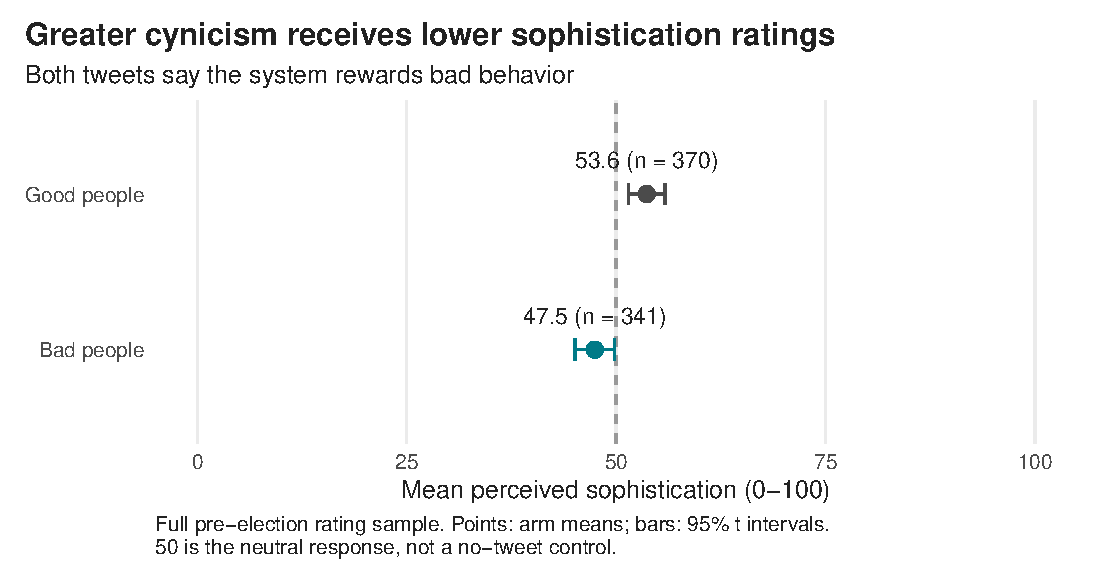
\includegraphics[width=\linewidth]{../figs/sophistication.pdf}
\caption{Perceived sophistication by tweet in the full rating sample. Means
and 95\% t intervals use all valid responses in each arm. The dashed line marks
the neutral response. The estimate of the between-arm contrast uses its own
standard error and does not rely on overlap of these arm intervals.}
\label{fig:means}
\end{figure}

\begin{table}[htbp]
\centering
\begin{tabular}{lrrr}
\toprule
Analysis & $n$ & Difference & 95\% interval \\
\midrule
Full sample & 711 & -6.2 & [-9.4, -3.0] \\
Covariate adjusted & 711 & -5.9 & [-9.2, -2.6] \\
Matched subset & 505 & -7.1 & [-10.9, -3.3] \\
Matched weighted & 505 & -7.9 & [-12.5, -3.3] \\
Rounded scale & 711 & -6.2 & [-9.4, -2.9] \\
Unmatched remainder & 206 & -3.9 & [-10.0, 2.1] \\
\bottomrule
\end{tabular}

\caption{Bad-people minus good-people ratings, in 0--100 scale points.
Intervals use Welch inference except for covariate-adjusted and weighted
estimates, which use HC3 t inference. The rounded scale uses
0, 16, 33, 50, 66, 83, and 100. Sample restrictions and weighting change the
target population; the rows are not independent replications.}
\label{tab:estimates}
\end{table}

The adjusted difference is \AdjustedEstimate{} points (\AdjustedCI{}).
Among the \MatchedRatingN{} rating respondents in the matched subset, the
unweighted difference is \SubsetEstimate{} (\SubsetCI{}); applying team weights
gives \WeightedEstimate{} (\WeightedCI{}). Inclusion in the matched subset is
\GoodRetention{}\% in the good-people arm and \BadRetention{}\% in the
bad-people arm. Similar retention rates do not establish selection on outcomes
is absent. The \RemainderN{} respondents excluded from the subset have an
estimated contrast of \RemainderEstimate{} (\RemainderCI{}), which is less
precise and compatible with both a negative difference and a modest premium.
The subgroup interval does not establish that exclusion changes the effect.

\subsection{Scale and influence checks}

Equal spacing is a convention for the rating scale. A binary comparison that
only asks whether a response is at least somewhat sophisticated gives a
\BinaryEstimate{} percentage-point difference (95\% interval \BinaryCI{}).
The six cumulative thresholds all have negative point estimates, although
several tail thresholds are imprecise (Table~\ref{tab:thresholds}). The
at-least-somewhat comparison has Holm-adjusted $p=\BinaryHolmP{}$ within that
six-test exploratory family. This pattern is not created solely by the
equal-spacing convention, but it does not establish population stochastic
dominance at every threshold.

Both sample medians are neutral. The probability that a randomly selected
bad-people rating exceeds a randomly selected good-people rating, counting a
tie as one half, is \RankProbability{}\%. A supplementary rank-sum test with
tie adjustment and continuity correction gives $p=\RankP{}$. This describes
the rating distributions, not the probability that an individual's rating
would fall under treatment.

A two-sided permutation check gives $p=\PermutationP{}$ using
\PermutationDraws{} draws, seed 20261004, and the finite-draw correction
$(k+1)/(B+1)$. Its approximate Monte Carlo standard error is
\PermutationMCSE{}. This test conditions on the observed arm sizes and assumes
complete random assignment within the rating route. The missing assignment
program prevents verification that this was the actual assignment mechanism.

Deleting each respondent in turn leaves the main contrast between
\LeaveMin{} and \LeaveMax{} points. Tables of leverage, design-matrix rank,
adjusted and weighted influence, and covariate balance are generated with the
analysis. The bounded outcome and complete item response limit the scope for
extreme-value and missing-outcome artifacts within the observed rating sample.

\section{Interpretation}

These estimates contradict a sophistication premium for the more cynical of
the two statements. Greater negativity about the people attracted to politics
is associated with lower perceived sophistication, and under random assignment
causes lower ratings in this sample. The direction persists across the full
sample, covariate adjustment, the supplied subset, and weighting. The evidence
supports that narrow finding, not a claim that every expression of cynicism
is penalized.

The result also differs from the perceived cognitive advantage of cynical
targets in \citet{stavrova2019}. It is not a direct replication: the present
comparison uses political statements that share criticism of incentives,
rather than contrasting generally cynical and noncynical people. It therefore
identifies a possible boundary to a broad sophistication-premium claim, without
overturning that study's evidence about other judgments and stimuli.

The separate belief sample provides context: \GoodBeliefPct{}\% select the
good-people statement and \BadBeliefPct{}\% the bad-people statement (the latter's
95\% interval is \BadBeliefCI{}). Because both choices criticize political
incentives, neither percentage measures how many people are cynical in a
general sense. More respondents endorse the statement that receives higher
sophistication ratings in the other sample. Agreement with the message could
help explain the rating gap, but no respondent has both outcomes, so these
files cannot test that mechanism or whether a person's own cynicism moderates
the contrast.

Exploratory treatment-interaction tests for gender, college education, age,
and Republican identity are imprecise (Table~\ref{tab:interactions}). Their
intervals admit substantively meaningful differences, so they do not establish
uniform effects. A direct test of the agreement mechanism would require
pre-treatment beliefs and subsequent ratings for the same respondents, with
the belief measurement timed to avoid priming the rating.

The main remaining design uncertainty is documentary: the full question stem,
randomization instructions, and verified stimulus display are absent. Those
materials would establish what was implemented. Additional stimuli varying
cynicism and perceived nuance separately would be needed to determine why
these statements differ and whether the result generalizes beyond them.

\bibliographystyle{plainnat}
\bibliography{references}

\appendix
\section{Response distributions and additional estimates}
\begin{figure}[H]
\centering
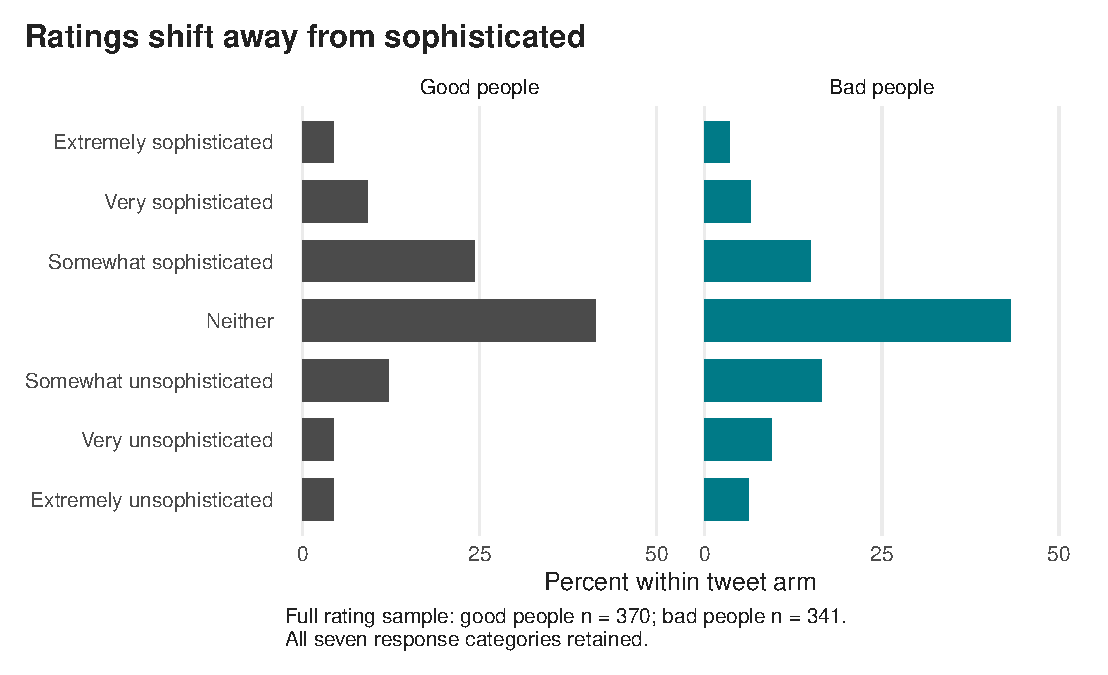
\includegraphics[width=\linewidth]{../figs/distribution.pdf}
\caption{All seven rating categories, expressed as percentages within each
tweet arm. The two panels use the same horizontal scale. Neutral responses remain
in the denominator.}
\label{fig:distribution}
\end{figure}

\clearpage
\section{Thresholds and interactions}
\begin{table}[H]
\centering\small
\begin{tabular}{lrrr}
\toprule
Sophistication threshold & Difference & 95\% interval & Holm $p$ \\
\midrule
Extremely & -0.8 & [-3.7, 2.1] & 0.5804 \\
Very or extremely & -3.5 & [-8.3, 1.2] & 0.4259 \\
At least somewhat & -12.9 & [-19.7, -6.1] & 0.0012 \\
At least neutral & -11.2 & [-17.6, -4.7] & 0.0038 \\
Above very unsophisticated & -6.9 & [-11.7, -2.1] & 0.0202 \\
Above extremely unsophisticated & -1.8 & [-5.1, 1.5] & 0.5505 \\
\bottomrule
\end{tabular}

\caption{Cumulative rating contrasts in percentage points, bad people minus
good people. All use the full rating sample and Welch intervals. Holm adjustment
applies to the six p-values; the displayed intervals are pointwise, not
simultaneous. ``Above'' excludes the named response and all less sophisticated
responses.}
\label{tab:thresholds}
\end{table}

\begin{table}[H]
\centering\small
\begin{tabular}{lrrr}
\toprule
Difference in tweet contrast & Estimate & 95\% interval & Holm $p$ \\
\midrule
Female minus male & -0.1 & [-6.7, 6.6] & 1.00 \\
College minus no college & 0.3 & [-6.4, 7.1] & 1.00 \\
Age 50+ minus under 50 & -1.1 & [-7.5, 5.4] & 1.00 \\
Republican minus other & 3.7 & [-3.9, 11.3] & 1.00 \\
\bottomrule
\end{tabular}

\caption{Exploratory differences in the tweet contrast, in 0--100 scale points.
Each row is a separate treatment-by-group interaction with HC3 t inference.
College means a four-year or postgraduate degree. Republican means the
Republican response in the five-category party item, without reallocating
leaners. Holm adjustment applies to these four tests. Intervals are pointwise.}
\label{tab:interactions}
\end{table}

\section{Reproduction}
Run \texttt{make restore} and \texttt{make check} from the repository root.
The pipeline reads the supplied SPSS files, validates their overlap and question
routing, writes aggregate tables, generates figures, compiles this report, and
runs lint and tests. The dependency lockfile records the R packages.
GitHub Actions runs the same checks.
Numerical prose is generated through \texttt{tabs/macros.tex}; tables and figures
use the same analysis outputs. No live data download is needed.

The tests independently reproduce Welch inference, derive weighted HC3
uncertainty from arm-level residuals, verify coding and denominators, test the
permutation correction, compare influence diagnostics with actual deletions,
and check recovery of known effects in simulated data. The data guide and
design note document every analysis variable and the interpretation assumptions.
\end{document}
